\documentclass{amsart}

\usepackage[]{enumerate} 
\usepackage[]{pst-platon} 
\usepackage[]{graphicx} 

\def\Gobble#1{}

\theoremstyle{plain}
\newtheorem{theorem}{Theorem}
\theoremstyle{definition}
\newtheorem{definition}{Definition}

\title{Euler's polyhedron formula}
\author{Ivar Haugal{\o}kken Stangeby}
\date{\today}

\begin{document}

\begin{abstract}
   In this short paper we look at Euler's polyhedron formula. This formula was
   one of my first experiences with more abstract mathematics, and I have loved
   it ever since. The proof is very simple, and extremely elegant.
\end{abstract}
\maketitle

\tableofcontents

\section{Introduction and motivation}
\label{sec:introduction_and_motivation}

As a vivid reader of popular science one often comes across the problem
regarding the \emph{Seven Bridges of K{\"o}ningsberg}. This city, located in
what was then known as Prussia had a river running through the middle. This
river naturally divided the city into the mainland --- on either side --- as
well as two large islands. Connecting these islands with the mainland were
seven bridges. This is where the famous question arises:

\begin{quote}
    \emph{Can the seven bridges of the city of K{\"o}ningsberg, over the river
    Preger, all be traversed in a single trip without doubling back and have
the trip end in the same place it began?}  
\end{quote}

Eminent mathematician Leonhard Euler proved that the problem stated above has
no solution. In working with the solution to this problem however, he dabbled
in a type of mathematics later to be known as \emph{graph theory}. One of the
more remarkable results (in my humble opinion) to arise from this new field of
mathematics is the discovery of a relationship between the number of vertices,
edges and faces in a polyhedron. It is exactly this relationship that Euler's
polyhedron formula captures.

\begin{theorem}[Euler's polyhedron formula]
    Any convex polyhedron's surface satisfies the equation
    \begin{equation}
        \notag
        V - E + F = 2
    \end{equation}
    where $V$, $E$ and $F$ denote the number of vertices, edges and faces,
    respectively.
\end{theorem}
\section{Preliminaries}
\label{sec:preliminaries}

In order to get a firm grasp of this formula, we first need to recall some
elementary geometry.  We start with the definition of the \emph{polyhedron}.

\begin{definition}[Polyhedron]
    A \emph{polyhedron} is a solid in three dimensions with flat polygonal
    faces, straight edges and sharp corners or vertices.\footnote{This
    definition is not very precice, but it will suffice for our purposes.}
\end{definition}

Polyhedra are named based on the number of faces using the greek prefix system.
Some examples include the \emph{hexahedron}, otherwise known as the cube with
its six faces; the \emph{octahedron} or \emph{double pyramid} with its eight
faces; and the \emph{icosahedron} with its 20 faces.

An important tool when studying platonic solids is that of the \emph{Schlegel
diagram}. It is essentially a way of projecting a $d$-dimensional object into
$d-1$ dimensions. In our case, we want to study the three dimensional platonic
solids in the two dimensional plane. Each platonic solid, when projected into
two dimensions, form what we call a \emph{planar graph}.

\begin{definition}[Planar graph]
  A \emph{planar graph}, is a graph that can be embedded in the plane, i.e., it
  can be drawn on the plane in such a way that its edges intersect only at
  their endpoints.
\end{definition}

\section{Proof of the formula}
\label{sec:proof_of_the_formula}

The proof of Euler's polyhedron formula is very simple and applies to any
convex polyhedron. We will use a cube as our example. We first take note of the
number of vertices, faces and edges. A cube has six faces, $F = 6$, twelve
edges, $E = 12$, and eight vertices, $V = 8$. This yields
\begin{equation}
    \label{eq:form}
    V - E + F = 8 - 12 + 6 = 2.
\end{equation}

Our goal now is to progressively remove edges, faces and vertices until we are
left with a very simple polygon. We will use transformations that preserve the
relation shown in equation \ref{eq:form}. We start by projecting the polyhedron
into the plane using a Schlegel diagram. This is done by removing one face and
squishing the cube into the plane, as shown in the leftmost image in figure
\ref{fig:proof}. Note that removing one face does not alter the number of
vertices and edges, hence we now have $V - E + F = 1$.

We now triangulate any face with more than three edges until all faces are
triangular. This is done by adding one edge, but doing so also adds a new face.
Hence the quantity $V - E + F$ is unchanged.

\begin{figure}[ht!]
    \centering
    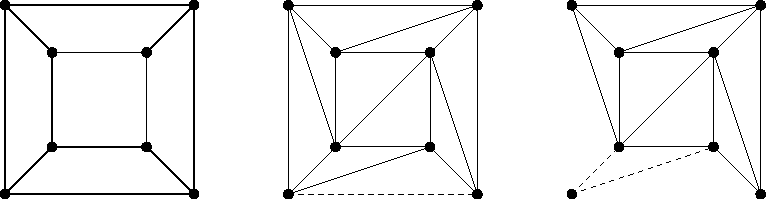
\includegraphics{drawing.pdf}
    \caption{First iterations of proof; using a cube.}
    \label{fig:proof}
\end{figure}

We now have two possible transformations to iterate: 
\begin{enumerate}
    \item Remove a triangle with one edge adjacent to the exterior as shown in
        the middle image in figure \ref{fig:proof}.  
    \item Remove a triangle
        with two edges adjacent to the exterior as shown in the rightmost image
        in figure \ref{fig:proof}.
\end{enumerate}
Note that neither of these operations change the quantity of interest. One
removes one edge and one face and the other removes one vertex, two edges, and
one face. We apply these transformations while always keeping the requirement
that the outer edges form a simple cycle. We will eventually end up with a
triangle with three vertices, three edges and one face.

\end{document}
